\documentclass[11pt]{article}
\usepackage[utf8]{inputenc}
\usepackage[T1]{fontenc}
\usepackage{graphicx}
\usepackage{booktabs}
\usepackage{amsmath}
\usepackage{amssymb}
\usepackage{hyperref}
\setlength{\emergencystretch}{2.5em}
\usepackage{geometry}
\geometry{a4paper, margin=2.5cm}
\usepackage{natbib}

\newcommand{\E}{\mathbb{E}}
\newcommand{\Prob}{\mathbb{P}}
\newcommand{\ind}{\mathbf{1}}

\title{CrystalRL --- Crystal Clear Reinforcement Learning:\\
\large from a Constrained Hierarchy to an Agent Legible by Construction}

\author{Ivan Pavliuk}
\date{Draft v0.4 --- July 2026}

\begin{document}
\maketitle

\begin{abstract}
Explaining a trading policy after it is trained does not make the policy readable. This paper
reports three generations of one system, in the order I built them, scored on a number that
could have come out against me. \textbf{CHRL}, a constrained hierarchical PPO trader, splits the
decision into three readable layers under five hard rules. It captures $93\%$ of the benchmark's Sharpe
ratio, its return per unit of volatility, at $52\%$ less drawdown. Its core is still a 64-dimensional unnamed latent vector with about $214$
tuning knobs. I then ran a dedicated post-hoc program over the frozen policy
(\textbf{Interpretable-CHRL}). It found a complete eight-primitive behavioral vocabulary, and
targeted edits of the hidden states and hidden actions survived matched-random controls
($+0.19$ to $+0.30$\,pp control-adjusted on a frozen 2022--23 rollout). The same program measured
where post-hoc explanation stops: a nine-rule story reproduced only $0.244$ of the deployed
policy's decisions, nothing bounds what a memory edit can touch, and steering is a correlation
rather than an intervention. \textbf{CRYSTAL-1} rebuilds the core so those limits go away. Memory
is a named regime posterior $b_t = \Prob(\text{bear}\mid\mathcal{F}_t)$ computed by an explicit
Bayes filter, the policy is a readable rule at full performance parity, and the command surface
is five named levers. On one scalar,
$\textsc{CrystalScore} = \text{Faithfulness}\times\text{Simulatability}\times\text{Stability}$
at a fixed $K{\le}9$ story budget, the agent moves from $0.15$ to $0.92$ on real market data, and
the entire gap is Simulatability. The certified readable rule,
``$b_t > 0.66 \Rightarrow$ exposure $0.74$'', held one-shot on 629 untouched trading days
(Sharpe $1.46$ vs $1.39$ buy-and-hold, max drawdown $-12.9\%$ vs $-15.5\%$). I close with what
all of this establishes about interpretable reinforcement learning in general: which axis
readable-by-design actually buys, why faithfulness probes can silently lie on threshold policies,
and where legibility is not free.
\end{abstract}

\section{Introduction: the question behind ``explainable''}
\label{sec:intro}

When a reinforcement-learning agent trades real money, someone always asks why it did what it
did. A regulator asks it, and I ask it every time I debug the system. In my companion work on
self-improving systems the question turns into a safety condition: \emph{an agent that changes
itself may only be allowed to do so to the degree it can be read}. The dominant practice answers
with post-hoc explanation: train a black box, then probe it. \citet{rudin2019} names the flaw.
For high-stakes decisions, do not explain the black box; build the model interpretable in the
first place. The critique is well known. What is scarce is a built system with a stated way of
measuring it: an agent made legible by construction, evaluated on real market data against a
strong black-box predecessor and against that predecessor's own best post-hoc program, with the
legibility difference expressed as a number all three can be scored on, and with the costs
stated.

\paragraph{The gap, stated with its sources.} The explainable-RL literature has declared its
own evaluation crisis. Successive surveys find evaluation ad hoc and non-comparable, with no
agreed faithfulness metrics and few human studies \citep{milani2024,vouros2023}.
\citet{kohler2025} state it plainly: there is ``no clear definition of policy
interpretability, i.e., no clear metrics'', human studies are costly, and interpretability is
routinely asserted without being measured. The metrics RL borrows from NLP are themselves under
indictment, since existing faithfulness tests have been shown to measure self-consistency rather
than faithfulness \citep{parcalabescu2024}, and saliency-style post-hoc evidence is exploratory
rather than explanatory \citep{atrey2020}. Meanwhile the belief-state line has descriptive
maturity and a prescriptive vacuum: recurrent policies provably approximate belief states
\citep{lambrechts2022}, yet no deployed policy I know of makes its belief a named, auditable,
\emph{writable} interface whose stated belief is certified to be the one it acts on.
\textbf{This paper answers all three. \textsc{CrystalScore} is an evaluation protocol that can
fail, applied identically to a black box, to its best post-hoc program, and to a
readable-by-design successor on one real high-stakes substrate, which is the instrument the
surveys ask for. Applying it yields the discriminating-axis finding: faithfulness does not
separate the architectures, parity-constrained simulatability does. And CRYSTAL-1's regime
posterior is, to my knowledge, the first certified named-and-writable belief interface of a
deployed policy (\S\ref{sec:crystal}).}

I present the work in the order I built it.\footnote{The paper's structure deliberately follows
three models: the system-paper arc of \citet{mnih2015} (problem $\to$ architecture $\to$ measured
evaluation $\to$ scope), the build-interpretable thesis of \citet{rudin2019}, and the
evaluation-rigor program of \citet{doshivelez2017}, whose taxonomy CrystalScore operationalizes.}
First I built the transparent-\emph{layers} agent (CHRL, \S\ref{sec:chrl}). Then I ran the
strongest post-hoc interpretability program I could over its frozen policy and measured both what
it buys and where it stops (\S\ref{sec:interp}). Then I rebuilt the core so the stopping point
disappears (CRYSTAL-1, \S\ref{sec:crystal}). Then I scored both architectures with one scalar
(\S\ref{sec:metrics}--\S\ref{sec:compare}). Everything that counts as evidence is computed on real
data. The one synthetic environment I built is used for instrument calibration only, behind an
explicit gate (\S\ref{sec:polygon}).

Contributions:
\begin{enumerate}
  \item \textbf{CHRL} (\S\ref{sec:chrl}): a constrained hierarchical PPO trader whose ablation
        shows that \emph{constraints, not hierarchy alone}, buy the risk-adjusted result, plus a
        precise measurement of where its transparency stops.
  \item \textbf{The post-hoc program} (\S\ref{sec:interp}): an eight-primitive behavioral
        vocabulary over the frozen policy, a taxonomy of controlled latent interventions, and
        control-adjusted evidence that targeted edits are real. This is the strongest case I can
        make \emph{for} post-hoc methods, and it is evidence against the thesis of this paper.
  \item \textbf{CRYSTAL-1} (\S\ref{sec:crystal}): named belief memory (an explicit Bayes
        filter), a readable-rule policy at parity, five named command levers.
  \item \textbf{CrystalScore and its measurement protocol} (\S\ref{sec:metrics}): faithfulness
        as intervention-following, simulatability as a parity-constrained short story,
        stability as seed replication, including a measurement correction (a faithfulness
        probe that silently lies on threshold policies) that is itself a finding.
  \item \textbf{The comparison} (\S\ref{sec:compare}): the identical scalar on both
        architectures, real data only, with the behavioral-influence toolbox (reward, teachers,
        interventions, architecture) exercised under controls.
  \item \textbf{The designed-market experiment} (\S\ref{sec:polygon}): can a market be built
        that rewards only a clean mind? Reported with the value-of-information gate that keeps
        its results out of market claims.
  \item \textbf{Conclusions for interpretable RL} (\S\ref{sec:conclusions}): five
        transferable findings and a falsifiable research program.
\end{enumerate}

\section{CHRL: how far do transparent layers go?}
\label{sec:chrl}

\subsection{Why a constrained hierarchy}
\label{sec:chrlwhy}

CHRL (Constrained Hierarchical RL) was my best answer to interpretability \emph{within} the
standard deep-RL recipe. Its design responds to three findings of the predecessor
feature-ablation study on the same market data: (i) feature quantity is not the bottleneck, since
a compact macro context outperforms broad feature stacks; (ii) cash must not be treated as just
another tradeable asset, because doing so lets the policy hide cash-heavy behavior inside an
opaque allocation vector; and (iii) the practical route to reading a trading policy is
\emph{logged, layered decisions}, not a monolithic end-to-end action. The design idea was
transparent behavior rather than a single action vector: factor the decision so that each stage
emits an observable, auditable signal.

Concretely, I split decisions into three layers on different rhythms, each readable on its own
timescale:
\begin{center}\small
\begin{tabular}{lll}
\toprule
layer & decision & rhythm \\
\midrule
risk & cash vs.\ risky exposure & ${\sim}20$ trading days \\
group & route capital through stock clusters & inherited context \\
stock & buy/sell candidate selection & ${\sim}5$ trading days \\
\bottomrule
\end{tabular}
\end{center}

The risk layer updates on a rhythm of about $20$ trading days and imitates a portfolio manager: PPO outputs the parameters of a Beta distribution, and a
draw from that distribution sets the split between cash and risky exposure. The group layer takes
that exposure as given and routes it across dynamic stock clusters, so the question of \emph{how
much} risk is settled before the question of \emph{where} it goes. The stock layer updates on a
rhythm of about $5$ trading days and imitates a trader: PPO outputs the parameters of a Dirichlet
distribution over the $29$ stocks in the universe, and a draw from it is the weight vector.

Five guardrails wrap the three layers, and each one is a rule the agent cannot break.
\emph{Exposure pacing}: the risk layer cannot flip the book from one day to the next.
\emph{Confidence-scaled sizing}: if the signal is weak, do not trade today. \emph{Event
triggers}: if the regime turns bear, de-risk, and re-open appetite only once recovery evidence
appears. \emph{Top-$K$ routing}: invest only in the top-$K$ names. \emph{Buy gate}: new risky
exposure is blocked until recovery evidence is visible. Hierarchy as a partial legibility device
has a long RL lineage \citep{sutton1999options,bacon2017option}; the guardrails are constraints of
the kind studied in safe policy optimization \citep{achiam2017}, imposed structurally rather than
through the reward. The core is a PPO policy \citep{schulman2017ppo} trained with the clipped
surrogate
\begin{equation}
L^{\text{CLIP}}(\theta) = \E_t\!\left[\min\!\big(\rho_t(\theta)\hat{A}_t,\;
\text{clip}(\rho_t(\theta),\,1{-}\epsilon,\,1{+}\epsilon)\,\hat{A}_t\big)\right],
\qquad \rho_t(\theta) = \frac{\pi_\theta(a_t \mid s_t)}{\pi_{\theta_{\text{old}}}(a_t \mid s_t)},
\label{eq:ppo}
\end{equation}
whose state $s_t$ passes through a 64-dimensional \emph{unnamed} latent.

The ablation that justifies the name is Figure~\ref{fig:chrlablation} and
Table~\ref{tab:chrlablation}: each panel of the figure is one metric, each bar one variant of the
model, and each table row the same variant. The concession comes first. The flat baseline is the
plain RL model, with no hierarchy and no rules. It has the
best raw return, $15.9\%$, and the best Sharpe, $1.14$, and it is also the riskiest arm: its worst
drawdown is $-14.8\%$ and it turns over $1.9\%$ of the book per day. I never claim to out-earn it.
My claim is the last column, return per unit of worst loss, where the full model is best at $1.37$
against the flat baseline's $1.08$. For a risk-managed product that is the number that matters.
Hierarchy \emph{alone} is the worst arm on that column ($0.79$, with $-13.0\%$ drawdown and
$1.8\%$/day turnover): structure without rules just adds churn. Constraints \emph{alone} do the
work on risk ($-6.3\%$ drawdown, $0.6\%$/day turnover) and pay for it in return ($8.2\%$). Only
the full combination recovers performance while keeping risk controlled (return/drawdown $1.37$,
the best of the four). The ingredient that carries the result is the constraint set. The hierarchy
is the scaffolding that makes the constraints expressible and the decisions loggable, and it pays
off only \emph{inside} them.

\begin{table}[h]
\centering\small
\begin{tabular}{lccccc}
\toprule
 & return & Sharpe & max drawdown & turnover (L1/day) & return/drawdown \\
\midrule
flat (neither)              & $\mathbf{15.9\%}$ & $\mathbf{1.14}$ & $-14.8\%$ & $1.9\%$ & $1.08$ \\
hierarchy only              & $10.3\%$ & $0.99$ & $-13.0\%$ & $1.8\%$ & $0.79$ \\
constraints only            & $8.2\%$  & $1.05$ & $\mathbf{-6.3\%}$ & $\mathbf{0.6\%}$ & $1.31$ \\
full CHRL (hier + constr)   & $10.0\%$ & $1.09$ & $-7.3\%$ & $0.8\%$ & $\mathbf{1.37}$ \\
\bottomrule
\end{tabular}
\caption{The four-way ablation on 4 walk-forward validation folds. Each row is one variant, best
per column in bold. The flat baseline keeps raw return and Sharpe, constraints own the risk
columns, and the full combination wins the ratio. Hierarchy alone is the \emph{worst} arm, so
constraints and not hierarchy buy the risk-adjusted result.}
\label{tab:chrlablation}
\end{table}

\begin{figure}[t]
  \centering
  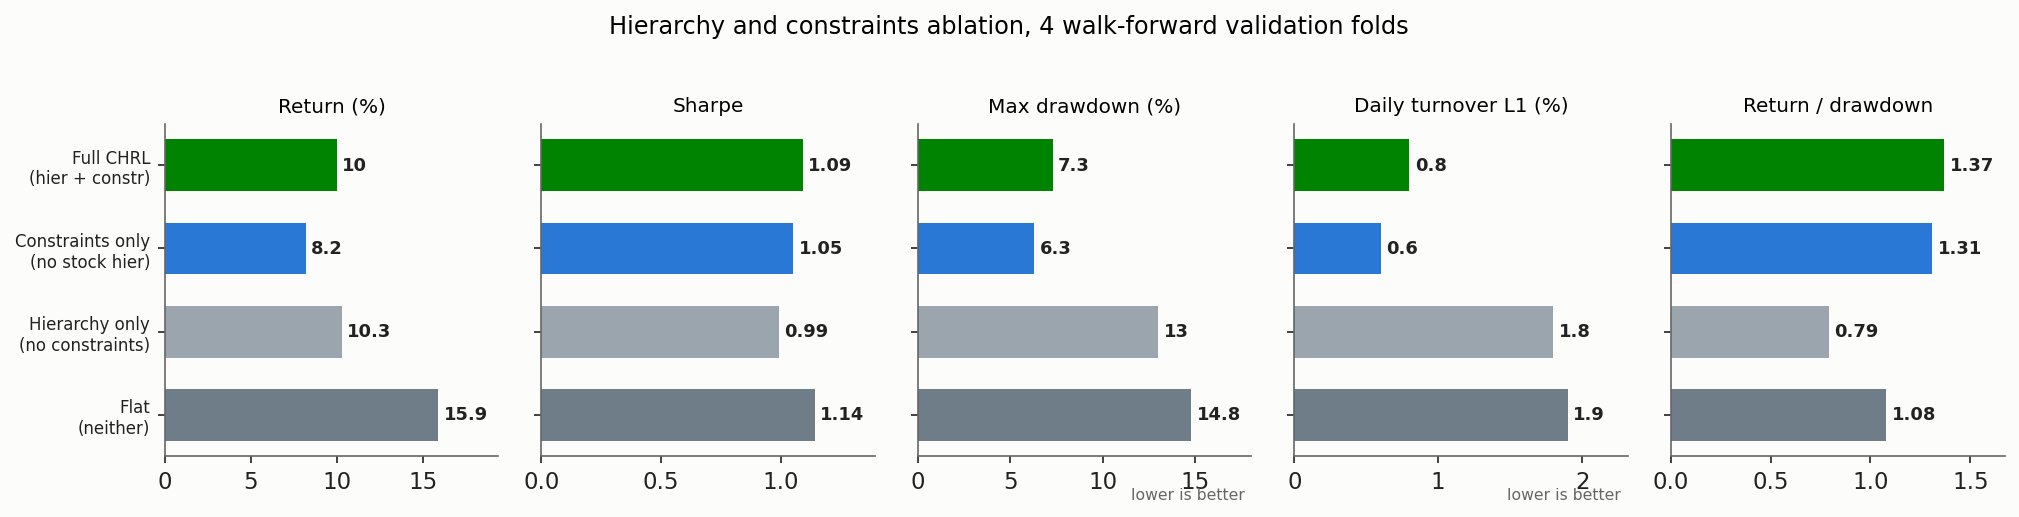
\includegraphics[width=\linewidth]{figures/fig_chrl_ablation.png}
  \caption{The same ablation, one panel per metric and one bar per variant. Constraints cut
  drawdown and turnover roughly in half, hierarchy alone hurts, and full CHRL recovers
  performance while keeping risk controlled.}
  \label{fig:chrlablation}
\end{figure}

\subsection{What it delivers}
\label{sec:chrlresults}

In four-fold walk-forward validation on the real US panel, CHRL delivers mean validation return
$10.05\%$, Sharpe $1.09$, max drawdown $-7.34\%$, mean cash weight $41.24\%$, and $0.84\%$/day
L1 turnover. Against the $100\%$-risky equal-weight universe benchmark (return $17.09\%$,
Sharpe $1.17$, max drawdown $-15.27\%$), it captures $93.2\%$ of benchmark Sharpe while cutting
drawdown by $52\%$. Its return-to-drawdown ratio is $1.37$ against the benchmark's $1.12$
(Figure~\ref{fig:chrl}). In plain language: a deliberately constrained agent gives up return to
buy a smoother ride and an auditable decision trail, which is the trade a risk-managed mandate
wants.

\begin{figure}[t]
  \centering
  \includegraphics[width=\linewidth]{figures/fig_chrl.png}
  \caption{CHRL. Left: the three-layer decision factorization and its five guardrails, where each
  stage emits a loggable, auditable signal on its own rhythm. Right: four-fold walk-forward
  validation against the $100\%$-risky equal-weight benchmark, showing $58.8\%$ of the return,
  $93.2\%$ of the Sharpe, and $52\%$ less drawdown.}
  \label{fig:chrl}
\end{figure}

So the layers are transparent, the guardrails are readable, and the trader is competent. The
question this paper turns on is the next one: \emph{what is the policy thinking between the
layers?}

\section{Reading the black box: the Interpretable-CHRL program}
\label{sec:interp}

Before replacing an architecture on interpretability grounds, I owed it the strongest post-hoc
reading I could produce. So I ran a dedicated program (Interpretable-CHRL) over the \emph{frozen}
trained policy, with no reward change, no re-optimization and no re-fit, asking one question with
increasing precision: \emph{which latent structures are actionable under controlled
intervention?}

\subsection{The staged pipeline}
\label{sec:stages}

The program runs in stages over a frozen rollout (Figure~\ref{fig:interp}, left). I log the
hidden states and action chunks. I \emph{discover} primitives by unsupervised clustering. I label
them behaviorally from the trading logs. I attach outcome diagnostics. Only then do I intervene.
The discovery stage yields a compact vocabulary with healthy statistics: a $K{=}8$ K-means
codebook with utilization $1.000$ (every primitive is used), perplexity $6.91$ (usage is spread
out, not collapsed onto a few codes), median run length $18$ trading days (primitives are
\emph{episodes}, not jitter), and cross-fold normalized mutual information $0.634$ (the vocabulary
largely replicates on held-out folds). The interventions themselves are one edit deep. I take the
policy's own hidden state $h_t$, push it along an interpretable direction $d$ with strength
$\alpha$, and pass the edited state through the \emph{original} frozen action head,
\begin{equation}
\tilde h_t \;=\; h_t + \alpha\, d, \qquad
\tilde a_t \;\sim\; \pi_\theta(\,\cdot \mid \tilde h_t\,),
\label{eq:intervene}
\end{equation}
so any behavioral change is attributable to the edit alone. I test five intervention families,
each phrased as a falsifiable question:
\begin{center}\small
\begin{tabular}{lp{10.2cm}}
\toprule
type & question \\
\midrule
suppression & does damping a locally harmful primitive improve the counterfactual rollout? \\
promotion & does amplifying a locally beneficial primitive improve it? \\
best-context map & does the best primitive depend on market regime (train-only target)? \\
replacement & does substituting a context-appropriate primitive for a weak one improve it? \\
repair & do a few targeted, context-conditional edits beat matched random alternatives? \\
\bottomrule
\end{tabular}
\end{center}

\subsection{What post-hoc buys, under controls}
\label{sec:interpresults}

The main methodological lesson arrived immediately. On this substrate a \emph{random-target
joint} edit (hidden state plus hidden action) also ``improves'' the frozen 2022--23 rollout, by
$+0.552$\,pp, because gentle noise perturbs a locally suboptimal policy off its habits. Every claim
below is therefore \emph{control-adjusted}: the reported value is the targeted edit's delta minus
its matched-random twin's (Figure~\ref{fig:interp}, right). Under that discipline three results
survive. First, hidden states are control surfaces: promoting a specific primitive yields
$+0.540$\,pp raw but $+0.263$\,pp control-adjusted ($+0.049$ Sharpe), and replacing a weak
primitive with its context-best alternative yields $+0.421$\,pp raw and $+0.302$\,pp adjusted.
Second, hidden \emph{actions} are control surfaces too: a learned adapter on the action pathway
gives $+0.377$\,pp raw and $+0.265$\,pp adjusted. Third, the effects are specific: adding targeted
repairs of two diagnosed primitives to the joint promotion baseline reaches $+0.508$\,pp where the
matched random-repair control reaches only $+0.316$\,pp, a specificity of $+0.192$\,pp. Post-hoc
analysis is not nothing. It found real, modular, editable structure inside a policy that was never
built to have any, and that result cuts against the thesis of this paper.

\begin{figure}[t]
  \centering
  \includegraphics[width=\linewidth]{figures/fig_interp.png}
  \caption{The Interpretable-CHRL program. Left: the staged pipeline over the frozen policy, which
  is log, discover ($K{=}8$ codebook; utilization $1.000$; perplexity $6.91$; median run $18$d;
  cross-fold NMI $0.634$), label, diagnose, intervene (Eq.~\ref{eq:intervene}), control. Right:
  the flagship counterfactuals on the frozen 2022--23 rollout, with each pair of bars showing raw
  against control-adjusted; the dotted line is the random-target joint edit ($+0.552$\,pp) that
  makes control adjustment mandatory.}
  \label{fig:interp}
\end{figure}

\subsection{Where post-hoc stops}
\label{sec:wall}

The same program measures its own ceiling, and every question I most cared about hit the same
wall. \emph{Memory}: the policy's state is smeared through the network, so nothing bounds what a
hidden-state edit can touch. The matched-random result above is exactly that symptom, since noise
moves behavior about as much as intention does, and only the \emph{difference} is knowledge.
\emph{Commands}: the control surface is about $214$ engineering knobs, none of which is a semantic
command. Steering means forcing the latent toward a post-hoc K-means centroid and checking that
behavior moves \emph{consistently}, which is a correlation and not an intervention.
\emph{Story}: when I scored the deployed agent's own stance log on the simulatability metric of
\S\ref{sec:metrics}, a $K{\le}9$ named story reproduced only $0.244$ of its behavior, so the
latent is genuinely incompressible at a human-story budget. \emph{Scope}: all counterfactual
evidence lives on one frozen, stress-heavy window (2022--23), because the frozen-policy discipline
that makes the measurements clean also chains them to a fixed rollout. The layers stayed
transparent and the core stayed opaque. The program's own stated next step, ``turn the
primitive-level signal into a cleaner training-time objective or policy-improvement loop'', is the
bridge this paper crosses: instead of discovering primitives after training, \emph{build the agent
out of named parts}.

\section{CRYSTAL-1: legible by construction}
\label{sec:crystal}

CRYSTAL-1 rebuilds the core around three commitments, each a direct answer to a measured
failure of \S\ref{sec:wall} (Figure~\ref{fig:arch}).

\paragraph{1. Memory is a named posterior.} The agent's only recurrent state is a belief over
$K$ market regimes, a point on the simplex $\Delta^{K-1}$, in the POMDP sense of a belief
state \citep{kaelbling1998}, over Hamilton-style regimes \citep{hamilton1989}. For the $K{=}2$
US machinery, with regime densities $f_z(r) = \mathcal{N}(r;\mu_z,\sigma_z^2)$,
$z\in\{\text{bull},\text{bear}\}$, and a sticky transition prior $\pi_{zz'}$, the belief is the
explicit Hamilton filter
\begin{align}
b_t \;=\; \Prob(z_t = \text{bear}\mid \mathcal{F}_t)
\;&=\; \frac{f_{\text{bear}}(r_t)\,\tilde b_t}
{f_{\text{bear}}(r_t)\,\tilde b_t + f_{\text{bull}}(r_t)\,(1-\tilde b_t)},
\label{eq:belief}\\
\tilde b_t \;&=\; \pi_{BB}\, b_{t-1} + \pi_{GB}\,(1-b_{t-1}),\nonumber
\end{align}
where $\mathcal{F}_t$ is the information available at $t$ (\S\ref{sec:data}). The word
\emph{named} does real work here. Because the coordinate has a meaning, a write to the belief is a
sentence (``believe bear at $0.8$''), and because $b_t$ is the sole memory channel, the blast
radius of any memory intervention is bounded by construction. That is the property
Eq.~\ref{eq:intervene} could test for but never guarantee.

\paragraph{2. The policy head is the story.} The decision layer is a small tree over
$[\,b_t,\ \text{inventory},\ \text{time}\,]$. In the soft form \citep{frosst2017} each inner
node $i$ routes by a sigmoid gate and each leaf $\ell$ holds a distribution over actions:
\begin{align}
p_i(x) &= \sigma\!\big(\beta(w_i^{\top}x + c_i)\big), \qquad
P^{\ell}(x) = \prod_{i \in \text{path}(\ell)} p_i(x)^{\ind[\ell \swarrow i]}
\big(1-p_i(x)\big)^{\ind[i \searrow \ell]},
\label{eq:tree}\\
\pi(a\mid x) &= \sum_{\ell} P^{\ell}(x)\, Q^{\ell}_a ,\nonumber
\end{align}
with the inverse temperature $\beta$ annealed so the trained tree is effectively hard. The
constraint is that the tree \emph{is} the policy, with no residual network for behavior to hide
in, and it must pay no performance tax (\S\ref{sec:compare}). At the limit the readable rule
degenerates to a sentence; the certified US rule of \S\ref{sec:cert} is literally
\begin{equation}
e_t \;=\; \begin{cases} 0.74, & b_t > 0.66\\[2pt] 1.00, & \text{otherwise,}\end{cases}
\label{eq:rule}
\end{equation}
where $e_t$ is the equity exposure.

\paragraph{3. Commands are few, named, and governed.} The roughly $214$-knob surface collapses to
\textbf{five agent-facing levers}:
\begin{center}\small
\texttt{SET\_BELIEF} \,\textperiodcentered\, \texttt{EXPOSURE\_MODE} \,\textperiodcentered\,
\texttt{GROUP\_CONCENTRATION\_CAP} \,\textperiodcentered\,
\texttt{ABSTAIN\_FLOOR} \,\textperiodcentered\, \texttt{DRAWDOWN\_BUDGET}
\end{center}
The concentration cap is \emph{hard}, which fixes the predecessor's soft-cap failure. Everything
else is engineering-fenced. A write is the \emph{do}-operator of \citet{pearl2009} made
concrete: $\texttt{SET\_BELIEF}(b^{*}, w)$ realizes
\begin{equation}
b_t \;\leftarrow\; (1-w)\, b_t + w\, b^{*}, \qquad w \in [0,1],
\label{eq:write}
\end{equation}
and a \emph{dose} nudge of $\delta$ nats acts in log-odds,
$\operatorname{logit}(b_t) \leftarrow \operatorname{logit}(b_t) + \delta$. Writes must pass a
non-inferiority bar on the certified objective before they are allowed to persist
(\S\ref{sec:compare}).

\begin{figure}[t]
  \centering
  \includegraphics[width=\linewidth]{figures/fig_architectures.png}
  \caption{The two architectures side by side. CHRL factors decisions into readable layers but
  keeps an unnamed 64-d latent core with about $214$ knobs, explained only after training
  (\S\ref{sec:interp}). CRYSTAL-1 makes the explanation the mechanism: a named belief as the
  sole memory channel, a readable rule as the policy itself, and five named command levers.}
  \label{fig:arch}
\end{figure}

\section{Data and evaluation}
\label{sec:data}

All quantitative claims are computed on real market data under point-in-time (PIT) discipline.
Two panels are used, and it matters which is which. CHRL, the post-hoc program over it, and the
exposure-rule experiments run on the lab's Dow-30 daily panel (2000--2026), which is where the
$29$ tradeable names of \S\ref{sec:chrlwhy} come from. The goal-planning machinery whose policy
tables the simulatability metric reads (\S\ref{sec:metrics}) runs on a menu of six liquid
US-listed assets plus cash: SPY (US large-cap equities), EFA (developed ex-US), IEF and TLT
(7--10y and 20y+ Treasuries), TIP (inflation-linked), GLD (gold), with the 13-week T-bill rate as
the cash leg. In both panels closes are split- and dividend-adjusted and converted to
total-return relatives, and the cash leg accrues $r^f_t = y_t/252$. Every panel enters through a signed data gate (file
hash, source URL, vintage recorded before any experiment may read it) and is ground-truthed
against an independent source. I added that last rule after being burned. A Chinese panel once
passed every internal consistency check while carrying a mixed clock, with close and volume
lagged a day against high and low. Only external ground-truthing caught it, and every result
computed on that panel was voided. A decision issued at $t$ may use only
$\mathcal{F}_t = \sigma(\{x_s : s\le t\})$, with publication lags respected; evaluation stands
at historical origins and is scored on realized continuations, never re-fit on them.

Two evaluation formulas recur. For a daily excess-return sequence $x_t$ and wealth path $W_t$:
\begin{equation}
\text{Sharpe} = \frac{\sqrt{252}\,\overline{x}}{\hat\sigma(x)}, \qquad
\text{max drawdown} = \min_{t}\Big(\frac{W_t}{\max_{s\le t} W_s} - 1\Big).
\label{eq:mdd}
\end{equation}
The goal-planning machinery that CRYSTAL-1 serves in production, which is scenario kernels by
stationary bootstrap \citep{politis1994}, dynamic programming on the funding ratio
\citep{das2020goals,browne1999}, and the promise backtests, is specified and evaluated in
the companion paper (\emph{Hello Crystal}). Here I use only its policy \emph{tables}, which
are the objects the simulatability metric reads.

\section{CrystalScore: measuring ``legible'' so it can lose}
\label{sec:metrics}

I want the legibility claim to be able to fail, so I score every architecture with
\begin{equation}
\textsc{CrystalScore} \;=\; F \times S \times S\!t,
\label{eq:cs}
\end{equation}
at a fixed parsimony budget $K \le 9$ (at most nine named rules or leaves), with each axis
operationalized so that it \emph{could have} come out low
\citep{doshivelez2017,jacovi2020,lipton2018}:
\begin{align}
F \text{ (faithfulness)} &= \E\Big[\ind\big[\pi\big(b \leftarrow \operatorname{do}(b^{*})\big)
= \pi^{*}(b^{*})\big]\Big],
\label{eq:faith}\\[3pt]
S \text{ (simulatability)} &= \operatorname{acc}\big(\text{story}_{K},\, \pi\big)
\ \ \text{s.t.}\ \ \big|\mathcal{R}(\text{story}_K) - \mathcal{R}(\pi)\big| \le \varepsilon,
\label{eq:simul}\\[3pt]
S\!t \text{ (stability)} &= \frac{1}{n}\sum_{i=1}^{n}
\ind\big[\text{mechanism replicates on seed } i\big].
\label{eq:stab}
\end{align}
Faithfulness (Eq.~\ref{eq:faith}): \emph{do}-writes must land, judged against a reference
optimum rather than against the policy's own habits. Simulatability (Eq.~\ref{eq:simul}): a
$K$-rule story must match the policy \emph{at performance parity} $\mathcal{R}$, because a story
that reproduces a lobotomized policy is cheating. Stability (Eq.~\ref{eq:stab}): the mechanism
must replicate across independent training seeds. The non-saturating companion is the \textbf{MDL
deficit} \citep{rissanen1978},
\begin{equation}
\Delta_{\text{MDL}} \;=\; \operatorname{Acc}(\pi) - \operatorname{Acc}(\text{story}_{K}),
\label{eq:mdl}
\end{equation}
which is the accuracy lost by forcing the explanation to be short. A value of $0$ means a short
story loses nothing.

\paragraph{A measurement correction, reported as a finding.} Faithfulness probes can silently
lie. My original probe applied fixed-size belief writes ($+0.2/+0.4$) and checked whether the
action followed. On threshold policies whose belief input saturates, such writes never cross
the decision boundary. So a policy that \emph{is} the rule by construction, a behavior-cloned
distillation with accuracy $0.97$, read $F{=}0.00$. The repaired protocol uses matched-state
\emph{contrast writes} ($b{=}0.2$ vs $b{=}0.8$, spanning both certified thresholds). Under the
corrected probe, cold-trained RL heads remain unfaithful under both probes ($F$ strict $0.00$,
contrast $0.00$), while teacher-warm-started heads score contrast-write $F = 0.77$--$0.83$ where
the strict probe read $0.03$ (\S\ref{sec:compare}). The general point is that an interpretability
metric is an instrument and needs a calibration surface. I caught this one on a designed
environment where the ground truth was known by construction (\S\ref{sec:polygon}).

\paragraph{Real-data values.} On its own deployed-panel stance log, the CHRL-line agent scores
$F{=}1.00$ (latent steering does move behavior, so faithfulness alone cannot distinguish the
designs), $S{=}0.244$ (\S\ref{sec:wall}), $S\!t{=}0.619$, giving
$\textsc{CrystalScore}{=}0.151$. CRYSTAL-1's axes on the real US machinery: $S{=}0.92$ (an
8-leaf tree reproduces the goal-planner champion's policy table at parity), $S\!t{=}1.00$ (the
certified rule's behavior replicates on 10/10 training seeds), $F{=}1.00$ (writing the bear
belief past the threshold changes exposure exactly as named), $\Delta_{\text{MDL}}{=}0.0$, giving
$\textsc{CrystalScore}{=}0.92$ (Figure~\ref{fig:crystalscore}). The entire $6\times$ gap is
Simulatability, which is what readable-by-design buys. Alpha does not enter the score.

\begin{figure}[t]
  \centering
  \includegraphics[width=.9\linewidth]{figures/fig_crystalscore.png}
  \caption{The identical scalar on both architectures, real data only. Each group of bars is one
  architecture and each bar is one axis of Eq.~\ref{eq:cs}. The CHRL line is scored on its own
  deployed-panel stance log; CRYSTAL-1 on the US goal machinery (tree-vs-champion simulatability)
  and the certified Dow rule (10-seed stability, write fidelity). Faithfulness is $1.0$ for both,
  because steering works on a black box too, so the discriminating axis is whether a $K{\le}9$
  named story can reproduce behavior at parity.}
  \label{fig:crystalscore}
\end{figure}

\section{The comparison: influence, certification, and the final table}
\label{sec:compare}

A legible agent is only useful if you can \emph{change} it on purpose. I exercised four
families of influence on CRYSTAL-1's PPO reward-dial heads, which are a research prototype and
not the champion, on the real US daily panel (train 2010--18, held-out evaluation after). Each
family came with a control battery, so what I report is what the levers actually do rather than
what they appear to do (Figure~\ref{fig:levers}).

\paragraph{R --- reward shaping.} The risk-targeted reward
\begin{equation}
r_t \;=\; e_t\, x_t \;-\; \lambda_{R}\,\max\big(0,\ \text{DD}_t - D^{*}\big)
\label{eq:reward}
\end{equation}
($e_t$ exposure, $x_t$ the asset return, $\text{DD}_t$ running drawdown, $D^{*}$ the budget)
moves the exposure dial, but the penalty \emph{alone does not enforce the budget}. Only the
$5\%$ head holds its budget, at $-4.81\%$ held-out max drawdown, and it does so by parking in
cash, while the $8\%$ and $12\%$ heads breach theirs ($-15.9\%$). A drawdown-matched twin shows
$z = 0.00$ timing skill, so reward shaping buys \emph{risk placement} and not timing. Enforcing
the budget requires a separate constrained objective: a Lagrangian head drives the breach down at
a $15$--$37$\,pp goal-probability cost. That is one more reason the transparent planner, which
respects capacity by a hard pre-filter, stays champion.

\paragraph{T --- teachers.} Trained cold, the heads' argmax behavior looked sensible while the
underlying preferences were nearly flat, an effectively untrained network masked by
deterministic evaluation (mean max action-probability $0.21 \approx 1/5$). The cure is behavior
cloning from the certified rule (Eq.~\ref{eq:rule}),
$L_{\text{BC}}(\theta) = -\E_{(s,a^{*})}[\log \pi_\theta(a^{*}\mid s)]$, at $87\%$ agreement, used
as a warm start \citep{ross2011dagger,rusu2016distillation}. Mean max action-probability goes from
$0.21$ to $0.73$, the belief starts to drive the action, and the corrected contrast-write probe
(\S\ref{sec:metrics}) shows the teacher installs the rule's \emph{causal} belief-to-action
structure ($F = 0.77$--$0.83$), which PPO fine-tuning does not erode on this substrate. Cold
discovery still fails; teaching works. (Leakage note: this teacher was \emph{selected} on the
2022--23 hold, so its hold read is contaminated. The leak-free teacher in the pipeline is the
planner champion, and a fresh read is pre-registered for 2027.)

\paragraph{I --- interventions, under controls.} This result overturns a first-pass claim of
mine. On the cold reward-dial heads, belief writes and per-primitive promotions \emph{appear}
to steer behavior. But a matched-random leaf moves behavior exactly as much as the targeted one,
so the placebo fails, and belief-write fidelity is $3\%$. The apparent steering was a
near-uniform-head artifact, which is precisely the failure mode \S\ref{sec:interpresults}'s
controls exist to catch. What survives is the refusal machinery: the certification gate correctly
refuses a $+1$-nat promotion that fails the non-inferiority test
\begin{equation}
\text{accept the write} \iff \widehat{J}_{\text{post}} \ \ge\ \widehat{J}_{\text{pre}} -
\delta_{\text{NI}},
\label{eq:ni}
\end{equation}
and it likewise rejects on the hold a reward ``winner'' selected on development ($z=1.34 < 2.15$).

\paragraph{A --- architecture.} Tree depth is a legibility dial set before training: depth-2
yields a 4-leaf policy, depth-3 the 8-leaf one. Scoring the prototype head itself, it is
perfectly simulatable ($S{=}1.0$, since a 4-leaf story distills the 8-leaf head exactly) and
stable ($S\!t{=}1.0$, 3 seeds), but when cold it is not faithful ($F{=}0.03$;
$\textsc{CrystalScore}{=}0.03$). That makes it a legible, stable \emph{dial} rather than a command
surface. The faithful command surface is either taught (lever T) or built (the champion's rule,
$F{=}1.0$).

\begin{figure}[t]
  \centering
  \includegraphics[width=\linewidth]{figures/fig_levers.png}
  \caption{The four influence levers on the real daily panel, under controls, one panel per lever.
  R: the reward penalty holds only the $5\%$ budget, so the penalty does not enforce the budget.
  T: the teacher warm-start cures the cold near-uniform collapse ($0.21\to0.73$; corrected
  contrast-write $F=0.77$--$0.83$). I: a matched-random leaf moves the cold head as much as the
  targeted one, so only the non-inferiority \emph{refusal} (Eq.~\ref{eq:ni}) survives. A: the
  cold head is a legible, stable dial ($S{=}1.0$, $S\!t{=}1.0$, $F{=}0.03$), not a faithful
  command surface.}
  \label{fig:levers}
\end{figure}

\subsection{A certified readable rule on untouched data}
\label{sec:cert}

The self-improvement loop's frozen certification gate (specified in the companion paper) has
certified exactly one real-data policy to date, and it is a sentence (Eq.~\ref{eq:rule}). It
entered with 7 accepts and \textbf{0} placebo accepts, and held one-shot on 629 untouched
trading days: Sharpe $1.46$ vs $1.39$ buy-and-hold, max drawdown $-12.9\%$ vs $-15.5\%$,
risk-adjusted improvement $z = +2.06$. The claim is a \emph{risk} claim, meaning the same return
with meaningfully less pain, and it is certified as such. A written return-improvement rule was
separately tested and closed ($-8.8\%$). I then audited the rule's machinery on the real panel:
naming faithfulness $1.0$ (the state called ``bear'' is the state in which de-risking is optimal
under the world model), 10-seed behavioral stability $1.0$, rule re-discovery from scratch $3/3$,
belief MDL deficit $0.0$. These are the CRYSTAL-1 entries of Figure~\ref{fig:crystalscore} and
Table~\ref{tab:final}.

\begin{table}[h]
\centering\small
\begin{tabular}{p{3.4cm}p{5.2cm}p{5.2cm}}
\toprule
 & \textbf{CHRL} & \textbf{CRYSTAL-1} \\
\midrule
Memory & 64-d unnamed latent, smeared; blast radius unboundable & named posterior $b_t$
(Eq.~\ref{eq:belief}); the sole memory channel \\
Policy legibility & post-hoc codes over a continuous latent; story acc.\ $0.244$ & the policy
\emph{is} a table/rule; 8-leaf story acc.\ $0.92$ at parity \\
Steering primitive & force the latent toward a K-means centroid (correlation; matched-random
controls mandatory) & named \emph{do}-write (Eq.~\ref{eq:write}), fidelity $1.0$ \\
Refusals & OOD gate shrinks or zeroes steps & the NI bar (Eq.~\ref{eq:ni}) refused a $+1$-nat
promotion \\
Control surface & ${\sim}214$ knobs & 5 named levers \\
Seed stability & $0.619$ & $1.00$ (10 seeds) \\
\textsc{CrystalScore} (Eq.~\ref{eq:cs}) & $\mathbf{0.151}$ & $\mathbf{0.92}$ \\
Flagship real-data result & walk-forward: Sharpe $1.09$, maxDD $-7.34\%$; control-adjusted
targeted edits $+0.19$--$0.30$\,pp & certified rule, 629 untouched days: Sharpe $1.46$ vs
$1.39$, maxDD $-12.9\%$ vs $-15.5\%$ \\
Deployment status & deployed: live firewall, operating history & goal machinery live on the US
universe (paper track); client certification still \emph{refused}, with dated unlocks \\
\bottomrule
\end{tabular}
\caption{The final comparison, real data only. Column by column: CHRL remains the
longer-operating deployed system and its post-hoc program found real editable structure;
CRYSTAL-1 wins every legibility and control axis and carries its own real-data results, while
its client-facing certification correctly refuses until the pre-registered reads mature.}
\label{tab:final}
\end{table}

\section{The designed-market experiment: can a market reward only a clean mind?}
\label{sec:polygon}

Real markets have very noisy logic. The regime is largely priced, so the honest value of even a
perfect regime belief can be zero, and a null result on real data cannot distinguish ``the
instrument is broken'' from ``there was nothing to detect.'' That motivates one deliberately
synthetic experiment: \emph{can I build a market that rewards only a ``clean'' mind, an
environment where the belief information carries value by construction, so that command-surface
machinery can be calibrated at all?}

I built such an environment, a regime market whose returns are generated from latent states
the belief can in principle track, and I used it strictly as \textbf{instrument calibration}.
On it, belief writes were \emph{proved} causal against an exogenous belief-MDP optimum
(agreement $0.80$/$0.835$ for the two heads). A likelihood-based \emph{lie detector} separates
sharp-but-wrong commands from uncertain-but-right ones (excess predictive NLL $0.43$ vs
${\approx}0$; detection $0.71$ at $5\%$ false alarms) while the na\"ive entropy gate points
\emph{backwards} and trusts the confident lie. A 216-cell factorial showed command composition
is non-additive with \emph{sign-flipping} cross-terms (median $|\varepsilon| = 2.66$), which is
why the write surface is governed by a calibrated ledger, a co-activation cap, a kNN manifold
governor ($24/24$ engineered off-manifold corners flagged at $1.2\%$ held-out FPR) and a writ
ladder with a first false-accept estimate ($0/48$; $\lesssim 6\%$ by the rule of three). On a
\emph{hard} designed substrate the gate also certified a genuine return-versus-legibility
\emph{tension}, so legibility is not free everywhere, and anyone claiming otherwise is measuring
easy tasks. This environment is also what exposed the faithfulness-probe blindness of
\S\ref{sec:metrics}.

The bridge back to reality is an explicit \textbf{value-of-information gate}
(Figure~\ref{fig:polygon}). The designed market shows VoI $= 5.92$, which is $+282\%$ of a
belief-blind baseline, and the gate \emph{opens}. On a real book the measured VoI is $0$ and the
gate \emph{closes}. So nothing calibrated on the designed market is allowed to generate a
real-market claim, and no designed-market number appears in \S\ref{sec:compare}.

\begin{figure}[t]
  \centering
  \includegraphics[width=.72\linewidth]{figures/fig_polygon.png}
  \caption{The designed-market experiment and its fence. Left: the environment built to reward
  a clean mind, where belief information is worth $+282\%$ of blind by construction, so command
  machinery (causal writes, the lie detector, composition governance, probe calibration) can be
  calibrated. Right: the same measurement on a real book returns zero, and the gate closes.}
  \label{fig:polygon}
\end{figure}

\section{What did not work, and what bounds the claims}
\label{sec:nulls}

A paper about honest machinery should list its own falsifications. Each of these cost me a
believed hypothesis, and the machinery that killed them is part of the contribution.
(i) \textbf{Raw counterfactual lifts were inflated about $2\times$}: a random-target joint edit
``improves'' the frozen rollout by $+0.552$\,pp (\S\ref{sec:interpresults}), so without matched
controls every post-hoc intervention result in \S\ref{sec:interp} would have been overstated.
(ii) \textbf{The strict faithfulness probe read $F{=}0.00$ on a policy that was the rule by
construction} (\S\ref{sec:metrics}), so an uncalibrated interpretability metric lied in the
pessimistic direction. (iii) \textbf{Cold RL heads are not command surfaces}: the placebo fails
and write fidelity is $3\%$, so only teaching or building installs causal structure
(\S\ref{sec:compare}). (iv) \textbf{A written return-improvement rule closed} at $-8.8\%$, so the
certified claim is risk-shaped and not alpha-shaped. (v) \textbf{A PPO challenger loses to the
readable planner table} on the same action space (regret $6.6$\,pp), which I report because the
field's default is the opposite claim. (vi) \textbf{Legibility is provably not free} on a hard
designed substrate (the certified tension of \S\ref{sec:polygon}). (vii) \textbf{Post-hoc
interpretability was not worthless}: it found the concepts that carried the result (motifs, codes,
counterfactual replay) that CRYSTAL-1 promoted from probes into architecture. The right summary is
that building them in made the story about $4\times$ more compressible, from $0.244$ to $0.92$ at
the same budget.

\section{Related work}
\label{sec:related}

Interpretability-by-construction vs post-hoc explanation \citep{rudin2019,lipton2018}; rigor
and evaluation of interpretability \citep{doshivelez2017,hoffman2018}; faithfulness as a
criterion \citep{jacovi2020}. Among the evaluation efforts of \S\ref{sec:intro}'s gap
paragraph, the program-distillation proxy of \citet{kohler2025} is the nearest. CrystalScore
differs in demanding intervention-grade faithfulness (per the self-consistency caution of
\citealp{parcalabescu2024}), performance-parity constraints on the story, and seed-replication
stability in one scalar. CRYSTAL-1's named belief is a concept-bottleneck design in the
sense of \citet{koh2020}, since the belief is a supervised, human-named intermediate through which
all memory must pass, with the difference that my bottleneck is also the \emph{write}
surface, so faithfulness is tested by intervention (Eq.~\ref{eq:faith}) and not only by probe
accuracy. Where circuit-style analysis \citep{olah2020} reverse-engineers named structure
\emph{out of} trained networks, CrystalRL builds the named structure \emph{in} and reserves
reverse-engineering for the audit. Belief-state control \citep{kaelbling1998} and regime models
\citep{hamilton1989} supply the named memory; soft trees \citep{frosst2017} the legible head;
MDL \citep{rissanen1978} the non-saturating ruler; interventional causality \citep{pearl2009}
the faithfulness protocol. Discretized latent-action behavior generation \citep{lee2024vqbet}
pursues the complementary direction, learned discrete codes for \emph{expressiveness}, where
CrystalRL fixes the codes to \emph{named} coordinates for legibility. Hierarchical RL as
partial legibility \citep{sutton1999options,bacon2017option}; PPO and constrained variants
\citep{schulman2017ppo,achiam2017}; goal-conditioned value functions \citep{schaul2015};
imitation-then-optimize \citep{ross2011dagger,rusu2016distillation}; reward shaping
\citep{ng1999shaping}; goal-based planning \citep{das2020goals,browne1999}; the stationary
bootstrap \citep{politis1994}. The self-improvement layer, which is LLM proposers over verified
evaluators \citep{romera2024funsearch,novikov2025alphaevolve,ma2023eureka,wang2023voyager} and
the statistics of adaptive search over noisy financial evaluators \citep{baileylopez2014dsr},
is treated in the companion paper (\emph{Hello Crystal}); this paper builds the object
those loops are allowed to modify.

\section{Conclusions: what this establishes about interpretable RL}
\label{sec:conclusions}

Five findings travel beyond this system.

\textbf{1. The discriminating axis is simulatability, not faithfulness.} Steering ``works'' on
a black box too ($F{=}1.0$ for both architectures). What readable-by-design buys is that a
$K{\le}9$ named story reproduces behavior at performance parity ($0.244 \to 0.92$). Evaluations
of interpretable RL that report only intervention success are measuring the wrong axis.

\textbf{2. Post-hoc analysis finds structure but cannot bound it.} The strongest post-hoc
program I could run found a real, complete, editable primitive vocabulary, and it still could
not bound the blast radius of an edit, name a command, or compress the policy into a story.
The two families are not rivals: post-hoc discovery told me \emph{which} concepts to build into
the successor.

\textbf{3. Controls and calibration are not optional.} A random-target edit improves the
rollout ($+0.552$\,pp), a placebo leaf moves a cold head as much as the targeted one, and a
strict faithfulness probe reads $0.00$ on a policy that is the rule by construction. Every
interpretability measurement in this paper that lacked a control or a calibration surface came
out wrong on the first pass, and in every case the error made the result look better than it
was.

\textbf{4. Causal command structure is taught or built, never free.} Cold RL training produced
legible, stable \emph{dials} with near-zero faithfulness. Behavior cloning from a certified
readable rule installed the causal belief-to-action structure ($F = 0.77$--$0.83$) and PPO
fine-tuning did not erode it. If you need a command surface, put it there on purpose.

\textbf{5. Legibility is not free everywhere, and where it is expensive is informative.} On
an easy substrate the readable rule pays no tax. On a hard designed substrate a certified
return-versus-legibility tension appears. The open question is \emph{where} the tension binds, not whether it exists.

The forward-looking program is falsifiable by design. Its flagship hypotheses: machine
simulatability predicts \emph{human} simulatability (kill: humans at chance while the machine
metric is at ceiling); a legibility scaling law, where optimal vocabulary size $K$ tracks
substrate behavioral complexity (kill: no relation across universes); interpretability
\emph{drift}, where naming faithfulness decays under a self-improvement loop unless re-certified
(kill: $F$ stays $1.0$ over 20+ accepted changes); motif conservation, where CHRL's discovered
primitives re-emerge as CRYSTAL-1 rule clauses (kill: no better-than-chance correspondence);
dose-response of \texttt{SET\_BELIEF} being monotone and saturating on certified substrates
(kill: non-monotone regions); the composition ledger's cross-terms appearing on the real panel's
visited manifold (kill of the premise: on-manifold interactions are additive); and CrystalScore
transferring to the \emph{improver}, where the coding agent's stated rationales predict its
measured effects (kill: rationale-effect agreement at chance, itself a publishable confabulation
result).

\section{Limitations}
\label{sec:limits}
(i) The scenario-based probabilities that the goal machinery quotes remain uncalibrated
research estimates; the calibration gates and their dated forward reads (2027-07-12; an
untouched multi-year fold maturing 2029) live in the companion paper. (ii) The real-data
CrystalScore's simulatability axis is measured on the planner champion and the certified rule
family, not yet on every head. (iii) The command-surface \emph{proofs} (causal writes
against an exogenous optimum, the lie detector, composition governance) are designed-market
calibrations (\S\ref{sec:polygon}); their real-data analogues are open hypotheses. (iv) All
Interpretable-CHRL counterfactuals live on one frozen, stress-heavy window (2022--23) by
design. (v) The certified rule is one rule family on one substrate; hardening across
substrates, seeds and profiles is the program's first milestone. (vi) Execution economics
beyond $10$\,bp switching costs (taxes, spreads, gaps) are only partially bounded.

\section*{Acknowledgments and drafting discipline}
Prepared \emph{write-paper-first} \citep{eisner-paper-first}. Experiments were run and logged
under the repository's honesty contract, where every entry names its null, its seed, and its worst
caveat, following \citet{feynman1974}: \emph{``The first principle is that you must
not fool yourself --- and you are the easiest person to fool.''} LLM coding agents (Claude,
Codex) operated the experimental loops under the stated controls, and every change they proposed
had to pass the fixed gates before it counted. The author thanks Joseph Lynch for discussions on
the interpretability track.

\bibliographystyle{plainnat}
\bibliography{refs}

\end{document}
